\chapter{Summationsnotation}
En summa av tal $a_1+a_2+...+a_n$ skrivs smidigare med summationsnotation:
\begin{equation*}
    a_1+a_2+...+a_n=\sum^n_{i=1} a_i
\end{equation*}
Indexet $i$ kallas för \underline{summationsindex} och existerar bara i själva summationen.
Summering är en linjär operation, dvs superpositionsprincipen gäller:
\begin{equation*}
    \sum_{i=1}^n(\alpha\cdot a_i+\beta\cdot b_i)=\alpha\sum_{i=1}^n a_i + \beta\sum_{i=1}^n b_1
\end{equation*}

Några viktiga standard summor är:
\begin{itemize}
    \item $\begin{matrix}
                  \sum_{i=1}^n 1= & \underbrace{1+1+...+1} & =n \\
                                  & n\text{ ggr}           &
              \end{matrix}$
    \item $\sum_{i=1}^n i=1+2+3+...+n=\frac{n\cdot(n+1)}{2}\text{ (aritmetisk)}$
    \item $\sum_{i=1}^n i^2=1^2+2^2+3^2+...+n^2=\frac{n(n+1)(2n+1)}{6}$
    \item $\sum_{i=1}^n r^{i-1}=1+r+r^2+...+r^{n-1}=\frac{r^n -1}{r-1},r\neq 1 \text{ (geometriskt)}$
\end{itemize}

Vill kunna beräkna arean under funktionsgrafer.
Strategin är att dela upp ytan i mindre bitar för vilka arean är lätt att beräkna och sedan summera alla bidrag.\\
%infoga bild 1
%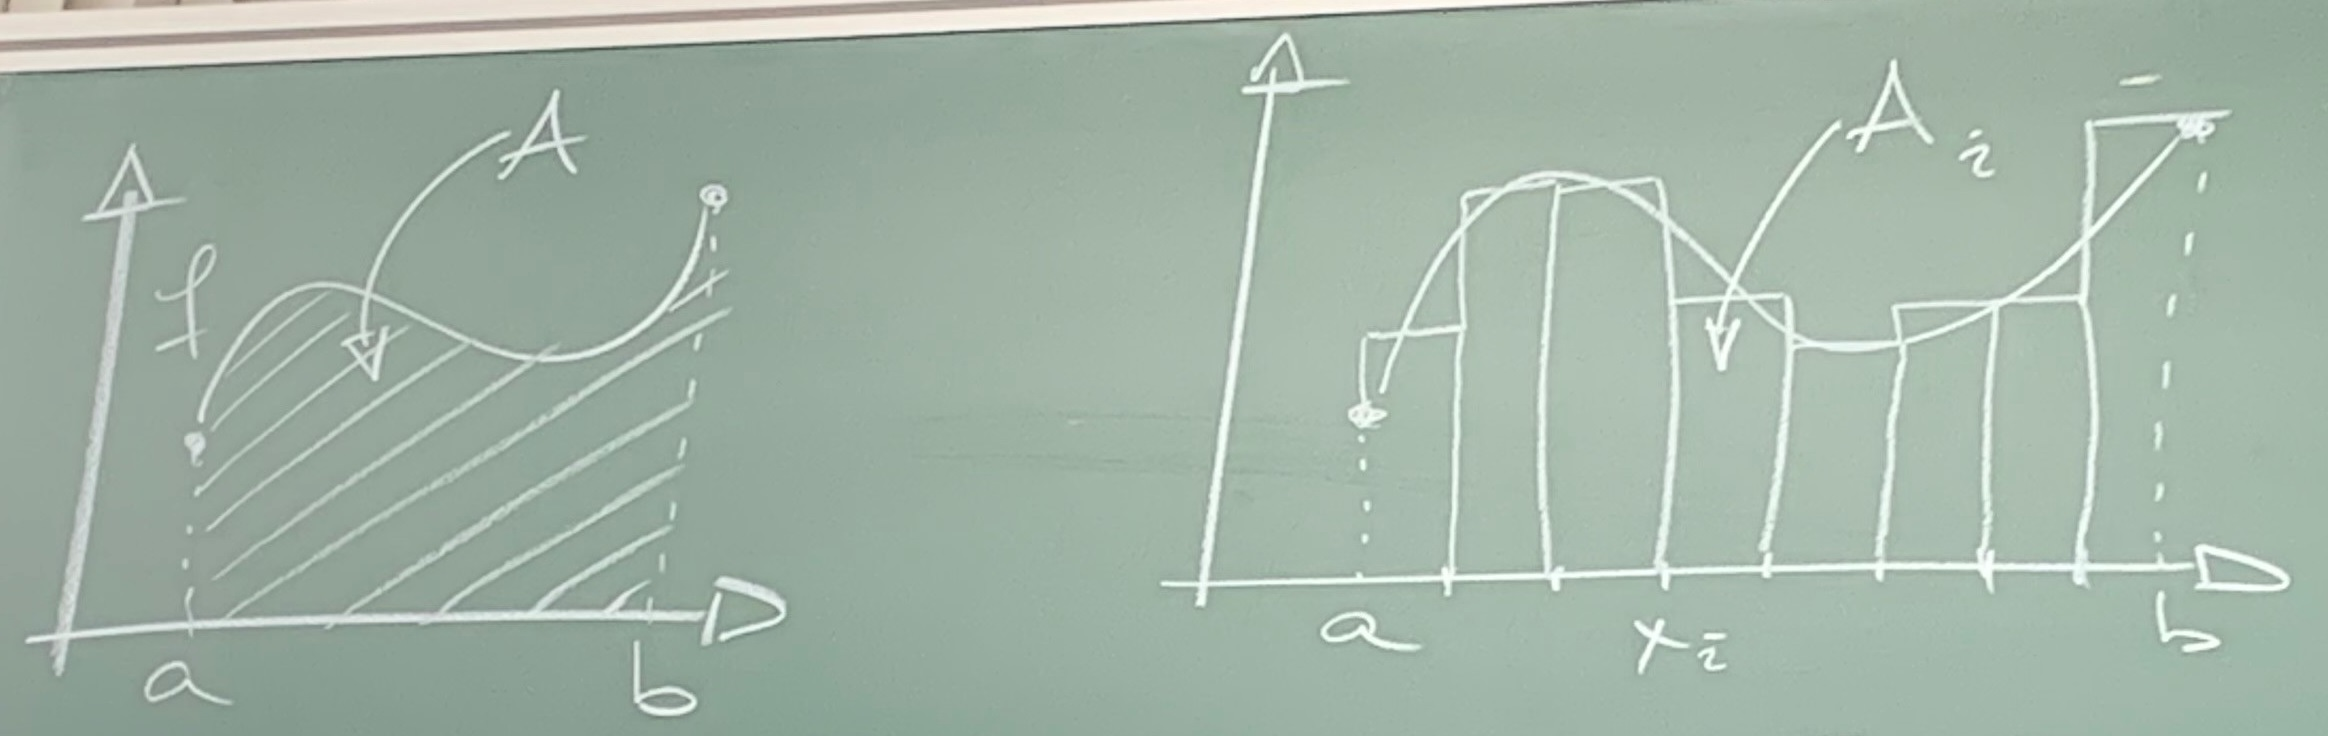
\includegraphics[scale=0.1]{lessons/lesson14/imgs/img01.jpg}
Dela upp intervallet $[a,b]$ i mindre delintervall med ändpunkter i $a=x_0<x_1<x_2<...<x_n=b$.
Varje delintervall är av bredden $\Delta x=x_1-x_0,\Delta x_2=x_2-x_1,$ osv.
Beräkna (t.ex) areorna av alla rektanglar med bred $\Delta x_i$ och höjd $\frac{f(x_i)+f(x_i+1)}{2}$ (medelvärdet).
Då borde $A\approx \sum_{i=0}^{n-1}\frac{f(x_1)+f(x_{i+1})}{2}\cdot\Delta x_i=\sum_{i=0}^{n-1} A_i$.
Approximationen \underline{borde} bli bättre och bättre i takt med att delintervallen blir mindre och mindre och det borde gälla att
\begin{equation*}
    A=\begin{matrix}
        lim        \\
        n\to\infty \\
        \Delta x_i\to 0
    \end{matrix}\sum_{i=0}^{n-1}A_i
\end{equation*}
Detta måste dock preciseras för att bli matematiskt relevant.

\paragraph{Ex (5.2.5)} Beräkna areorna under grafen till $y=x^2$ mellan $x=1$ och $x=3$.
\subparagraph*{Lösning}
%infoga bild 2
%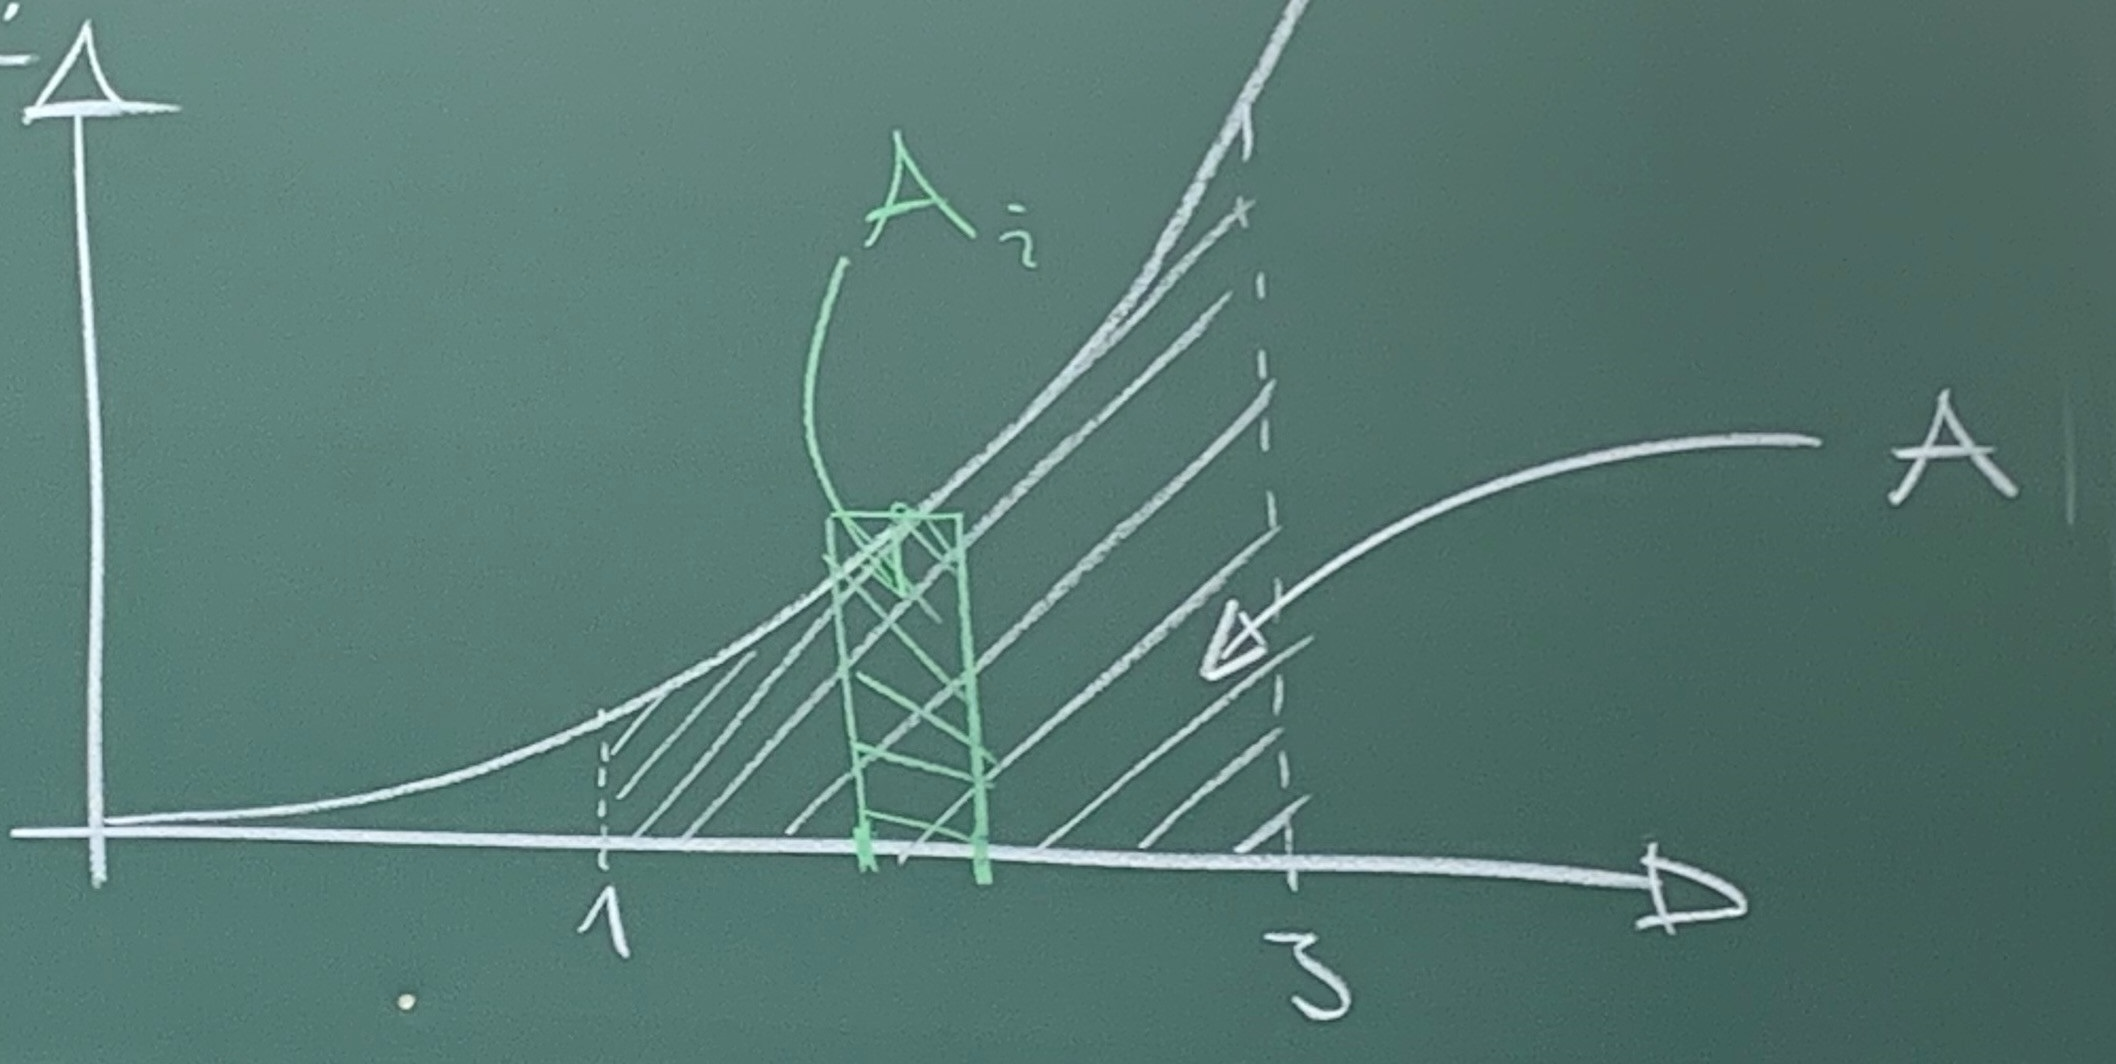
\includegraphics[scale=0.1]{lessons/lesson14/imgs/img02.jpg}
Dela upp intervallet $[1,3]$ i $n$ stycken lika stora delar.
Delintervallets bredd blir då $\Delta x=\frac{3-1}{n}=\frac{2}{n}$ med ändpunkter i $1,1+\frac{2}{n},1+2\frac{2}{n},...,1+(n-2)\frac{2}{n},3$.
Om vi använder funktionens medelvärde i varje delintervall som höjd för att approximerande rektanglar får vi att:
\begin{equation*}
    A=\lim_{n\to\infty}\sum_{i=1}^n \frac{f(x_i)+f(x_{i-1})}{2}\cdot\delta x=
    \lim_{n\to\infty}\sum_{i=1}^n \frac{(1+i\cdot\frac{2}{n})^2+(1+(i-1)\frac{2}{n})^2}{2}\cdot\frac{2}{n}=
\end{equation*}
\begin{equation*}
    \lim_{n\to\infty}\sum_{i=1}^n\frac{1+\frac{4i}{n^2}+\frac{4i^2}{n^2}+1+\frac{4i}{n}-\frac{4}{n}+\frac{4i^2}{n^2}-\frac{8i}{n^2}+\frac{4}{n^2}}{2}\frac{2}{n}=
    \lim_{n\to\infty}\sum_{i=1}^n\frac{2}{n}+\frac{8i}{n^2}+\frac{8i^2}{n^3}-\frac{4}{n^2}-\frac{8i}{n^3}+\frac{4}{n^3}=
\end{equation*}
\begin{equation*}
    \lim_{n\to\infty}(\frac{2}{n}\cdot n+\frac{8}{n^2}\cdot\frac{n(n+1)}{2}+\frac{8}{3}\cdot\frac{n(n+1)(2n+1)}{6}-\frac{4}{n^2}\cdot n-\frac{8}{n^3}\cdot\frac{n(n+1)}{n}+\frac{4}{n^3}\cdot n=
\end{equation*}
\begin{equation*}
    2+4+\frac{16}{6}=6+\frac{8}{3}=\frac{26}{3}\text{ a.e }\Box
\end{equation*}
~\\
För att areaberäkning genom approx. med staplar ska vara "vettig" mpste det gälla att resultatet är oberoende av:
\begin{enumerate}
    \item hur $x$-axeln styckas upp
    \item vilken stapelhöjd som väljes i varje delintervall (dvs overoende av $f(s)$ där $s\in[x_i,x_{i+1}]$)
\end{enumerate}
En uppdelning av ett intervall $[a,b]$ i disjunkta delintervall $[x_0,x_1],(x_1,x_2],...,(x_{n-1},x_n]$ kallas för en \underline{partition} av $[a,b]$ och kan refereras till som mängden av ändpunkter:
\begin{equation*}
    P=\{x_0,x_1,...,x_n\}
\end{equation*}
Varje delintervall i $P$ har en längd $\Delta x_i=x_{i-1}-x_i$ och man definierar \underline{normen} som längden av det längsta delintervallet:
\begin{equation*}
    ||P||:=\begin{matrix}
        \text{max} \\
        1\leq i \leq n
    \end{matrix}\Delta x_i
\end{equation*}
Om $f$ är en kontinuerlig funktion så antas både ett maximalt och ett minimalt värde någonstans i varje delintervall, säg i $x=u_i$ och $x=l_i$ för delintervallet $[x_i,x_{i+1}]$.
% infoga bild 3
%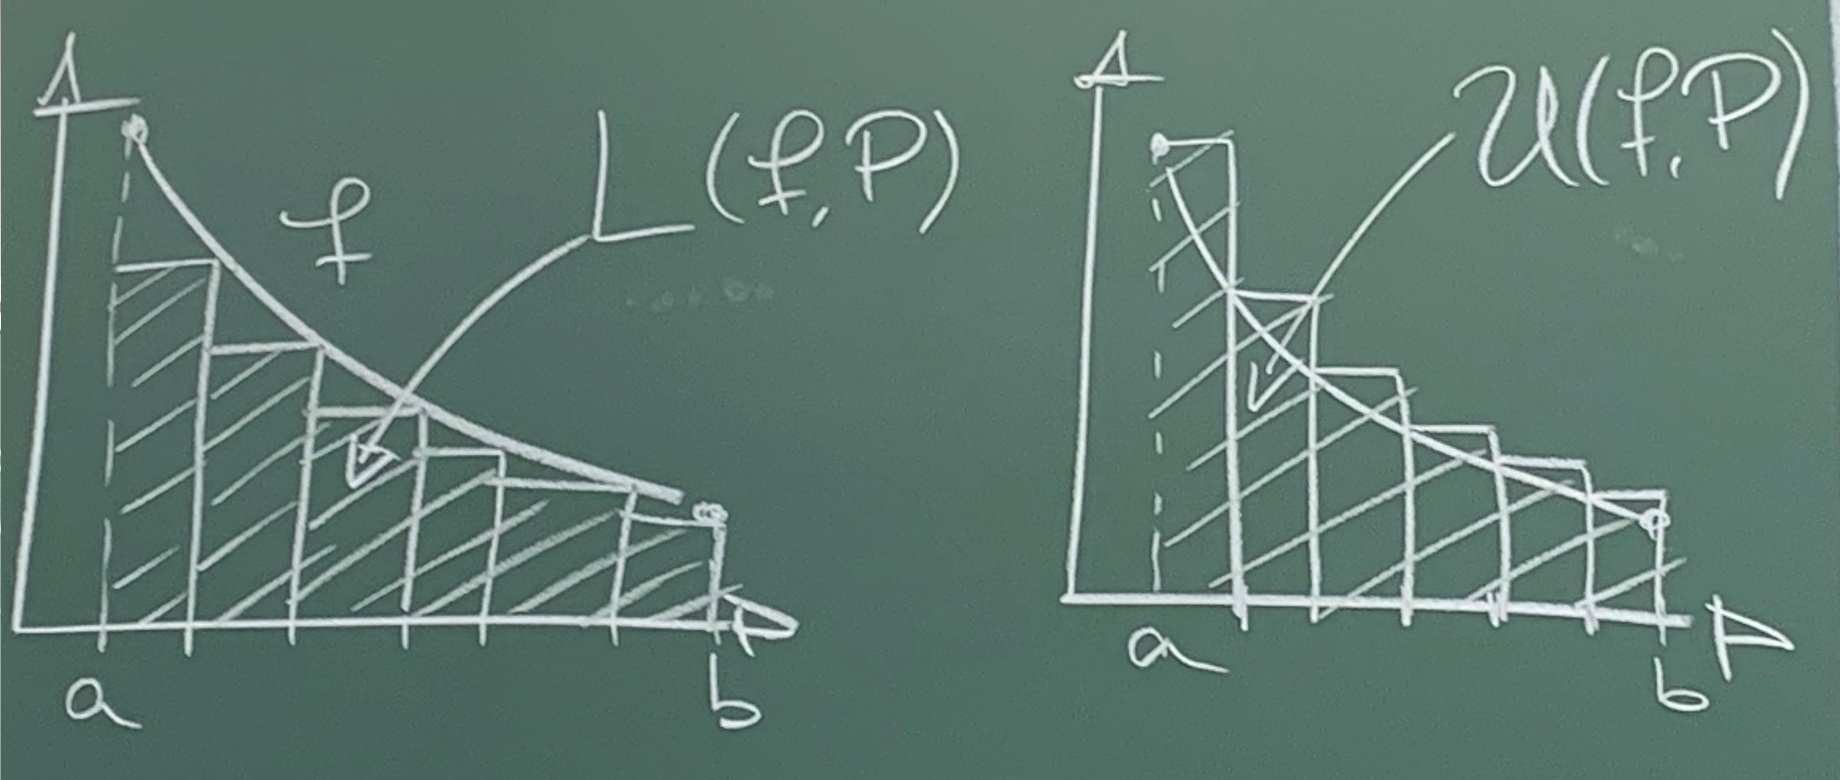
\includegraphics[scale=0.1]{lessons/lesson14/imgs/img03.jpg}
Dvs. om $x\in[x_i,x_{i+1}]$ så gäller att $f(l_i)\leq f(x)\leq f(u_i)$.
Det betyder att en godtycklig stapel över intervallet $[x_i,x_{x+i}]$ \underline{alltid} kommer att ha en area $A_i$ så att
\begin{equation*}
    f(l_i)\cdot\Delta x_i\leq A_i\leq f(u_i)\cdot\Delta x_i
\end{equation*}
Givet en partition $P$ kan vi definiera den nedåt begränsande Riemann-summan $L(f,P)$ och den övre begränsande $U(f,P)$ som:
\begin{equation*}
    L(f,P)=\sum_{i=1}^n f(l_i)\cdot\Delta x
\end{equation*}
\begin{equation*}
    U(f,P)=\sum_{i=1}^n f(u_i)\cdot\Delta x
\end{equation*}
%infoga bild 4
%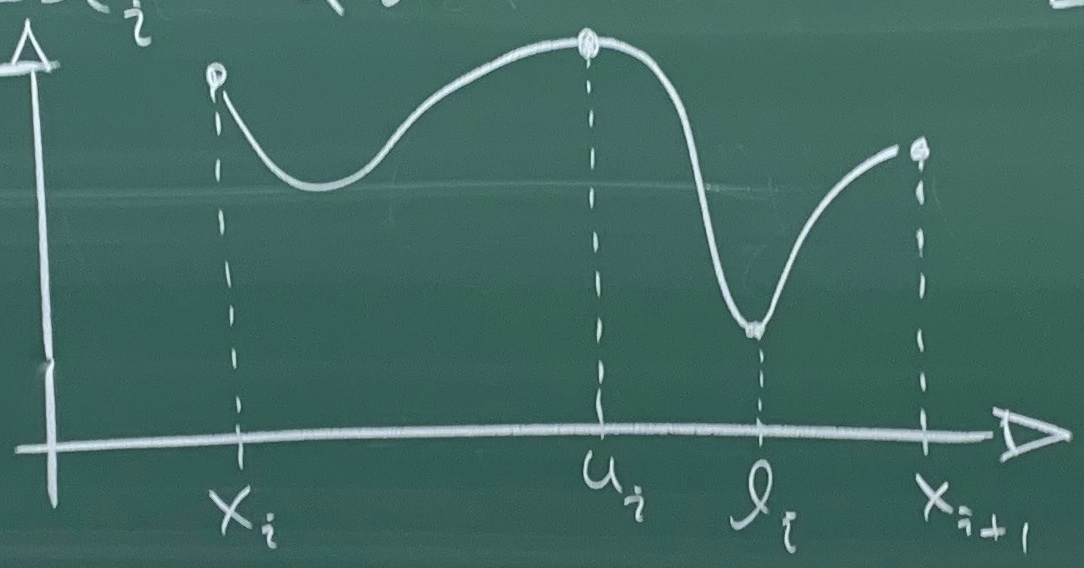
\includegraphics[scale=0.1]{lessons/lesson14/imgs/img04.jpg}
Om $f$ beter sig "vettigt" och $P$ blir en finare och finare partion av intervallet $[a,b]$ där $||P||\overrightarrow{n\to\infty}0$ så \underline{borde} $\lim_{n\to\infty}L(f,P)=\lim_{n\to\infty}U(f,P)$ oavsett val av partition $P$.
I så fall är det ett rimligt mått av arean under funktionsgrafen.
Detta definierar den \underline{definita intergralen} av $f$ mellan $a$ och $b$.

\paragraph{Definition (definit integral) (tenta)} Antag att det finns precis ett enda tal $I$ så att det för varje partition $P$ av $[a,b]$ gäller att: $L(f,P)\leq I\leq U(f,P)$\\
I så fall säger man att $f$ är \underline{intergrerbar} över $[a,b]$ och vi kallar talet $I$ för den \underline{definita integralen} av $f$ över $[a,b]$.
Detta skrivs symboliskt som
\begin{equation*}
    I=\int_{a}^{b} f(x) \,dx
\end{equation*}
Notera att $\int_{a}^{b} f(x) \,dx$ är ett \underline{tal} och inte en funktion.
"Variabeln" $x$ existerar endast inuti integralen och kallas för \underline{integrationsvariabel}.
Talen $a$ och $b$ kallas nedre- och övre-integransgräns.
Funktionen $f$ kallas för \underline{integrand} och $dx$ för \underline{differntialen}.


Definierade utifrån Riemann-summor är en hörnsten inom matematisk analys tillsammans med definitionen av derivatan och definitionen av gränsvärde.
Räcker gott och väl för praktiska tillämpningar men ej för vidare teoretiskt arbete (då används Lebesque integralen).